\documentclass{scrartcl}
\usepackage[utf8]{inputenc}
\usepackage[T1]{fontenc}

% Für schöneren Blocksatz
\usepackage{microtype}

% Für deutsche Sprache
\usepackage[ngerman]{babel}

% Für deutsche Zitate / Anführungszeichen
\usepackage{csquotes}

% Für Quellenangaben
\usepackage[sorting=none, defernumbers=true]{biblatex}
\addbibresource{sources.bib}

% Für klickbare links (Kasten werden nicht mitgedruckt)
\usepackage{hyperref}

% Für Zusammenfassung
\usepackage{abstract}

% Für das Einfügen von Bildern
\usepackage{graphicx}

% Für wrapfigure (Text um Bilder herum)
\usepackage{wrapfig}

% Für custom captions
\usepackage{caption}
\captionsetup{textfont={footnotesize}, labelfont={footnotesize, bf}, position=below, format=plain}

% Für \affil
\usepackage{authblk}

% Für Kopf-/Fußzeilen
%\usepackage{scrlayer-scrpage}
% \renewcommand*{\headfont}{\normalfont}
%\setkomafont{pagehead}
%\rehead[]{JUGEND FORSCHT -- PROJEKTBERICHT}
%\rohead[]{JUGEND FORSCHT - PROJEKTBERICHT}


\usepackage{fancyhdr}
\fancyhf{}
\pagestyle{fancy}
\fancyhead[R]{JUGEND FORSCHT -- PROJEKTBERICHT}
\fancyfoot[C]{\thepage}


% Für Seitenränder
% \usepackage{geometry}
% \geometry{left=2.5cm, right=2.5cm, top=2.5cm, bottom=2cm}

\title{\textbf{\Huge 
\texttt{
	Erkennung ereigniskorellierter Potenziale eines Elektroenzephalogramms durch eine KI
}
} \\ \vspace{20mm}}

\date{}
\author[]{\textbf{\huge Alexander Reimer und Matteo Friedrich}}
\affil[]{\textbf{\LARGE Gymnasium Eversten Oldenburg} \\ \vspace{10mm} \textbf{\Large Betreuer: Herr Dr. Glade \& Herr Husemeyer}}

\begin{document}

	\newcommand{\sig}{\textrm{sig}}
	\newcommand{\netin}{\textrm{netzinput}}

	\newcommand{\threesub}[1]{
	\vspace{1.5ex}
	\noindent {\textbf{#1}}
	\vspace{0.5ex}
	}

	\maketitle

	\newpage
	
	\tableofcontents
	
	\newpage

	\section{Zusammenfassung}


	In diesem Projekt wollen wir einen Roboter mithilfe bloßer Gedankenkraft steuern.

	Um Daten über das Gehirn zu bekommen, nutzen wir einen Elektroenzephalographen, kurz EEG, welches durch Elektroden an der Kopfhaut die Spannungsdifferenz innerhalb des Gehirns misst. Dies werten wir mithilfe eines Neuronalen Netzes aus, welches wir vorher darauf trainiert haben, Muster in diesen Daten zu erkennen. So können wir bestimmte Ereignisse anhand der EEG-Daten ableiten, z.B. ob jemand geblinzelt hat oder sich gerade konzentriert.
	
	Das Ziel ist es dann, durch das Erkennen verschiedener dieser sogenannten ereigniskorrelierten Potentialen (EKPs) einen Roboter nur mit Gedanken steuern zu können.
	
	
	Wir haben es geschafft eine KI zu programmieren, die in der Lage ist, anhand der EEG-Daten richtig zu erkennen, ob eine bestimmte Testperson gerade geblinzelt hat oder nicht. Diese korrekte Klassifizierung der Daten ist jedoch nur möglich, wenn die Test- und Trainingsdaten unter den exakt gleichen Voraussetzungen aufgenommen wurden (das heißt gleiche Person, gleiche Umgebung etc.) Diese Problematik könnten wir wahrscheinlich durch das Sammeln von mehr und verschiedenen Daten lösen. Leider hatten wir dafür aber noch nicht genug Zeit gehabt.	

	\section{Einleitung}
 
	Ziel des Projektes ist es, zuerst ein BCI -- Brain-Computer Interface -- zu entwickeln, welches verschiedene EKPs erkennen kann. Dieses wollen wir dann testen, indem wir es zur Steuerung eines Roboters nutzen.

	Die Idee eines BCI ist nicht neu, sondern wird intensiv erforscht. Aufgrund bereits durchgeführter Experimente ist bekannt, dass BCIs umsetzbar sind. \cite{BCIChaudhary}
	
	Wir hoffen, neben dem Erlangen von Erfahrung in diesem interessanten Bereich auch selbst dazu beizutragen. Dies wollen wir erreichen durch das Entwickeln einer allgemeinen Anwendung, bei der kein vorheriges Trainieren für eine fremde Person benötigt wird, das Umsetzen mit günstiger, für viele bezahlbarer Hardware, sowie ein performantes Programm, welches leicht für die eigenen Zwecke anpassbar ist.

	\newpage

	\section{Methode und Vorgehensweise}

	\subsection{Materialien} \label{Materialien}

	\begin{itemize}
		\item EEG
		\begin{itemize}
			\item 4 Channel Ganglion Board von OpenBCI $\star$
			\item 2x Spike und 2x Flat Electrodes  $\star$
			\item Klettband für die Elektroden $\star$
			\item 2x Earclips $\star$
			\item Lithium-Polymer-Akku und Ladegerät $\star$
			\item Plastik-Hülle für das Ganglion Board
		\end{itemize}

		\item Roboter
		\begin{itemize}
			\item Lego Mindstorms EV3 Brick
			\item Raspberry Pi 3B 8GB
			\item 2x EV3 großer Motor
			\item SD-Karte (8 GB)
			\item Diverse Legoteile
		\end{itemize}

		\item Software
		\begin{itemize}
			\item Flux.jl für das neuronale Netz
				\footnote{\href{https://github.com/FluxML/Flux.jl}{https://github.com/FluxML/Flux.jl}}
				\cite{Flux.jl-2018}
				\cite{innes:2018}
			
			\item BrainFlow.jl als Schnittstelle zum EEG
				\footnote{\href{https://github.com/brainflow-dev/brainflow}{https://github.com/brainflow-dev/brainflow}}
				\cite{brainflow}
			
			\item FFTW.jl für die Fast Fourier Transformation
				\footnote{\href{https://github.com/JuliaMath/FFTW.jl}{https://github.com/JuliaMath/FFTW.jl}}
				\cite{FFTW.jl-2005}
			
			\item CUDA.jl zum effektiven Nutzen einer NVIDIA GPU
				\footnote{\href{https://github.com/JuliaGPU/CUDA.jl}{https://github.com/JuliaGPU/CUDA.jl}}
				\cite{CUDA}
			
			\item PyPlot.jl zum plotten
				\footnote{\href{https://github.com/JuliaPy/PyPlot.jl}{https://github.com/JuliaPy/PyPlot.jl}}
				\cite{pyplot}
			
			\item BSON.jl zum Speichern und Laden von Netzwerken
				\footnote{\href{https://github.com/JuliaIO/BSON.jl}{https://github.com/JuliaIO/BSON.jl}}
			
			\item ev3dev.jl zum Steuern eines EV3-Roboters durch einen Raspberry Pi
				\footnote{\href{https://github.com/AR102/ev3dev.jl}{https://github.com/AR102/ev3dev.jl}}
				\cite{ev3dev}
			
		\end{itemize}

	\end{itemize}

	\subsection{Vorgehensweise}

	Unser Projekt lässt sich grob in 3 Teile unterscheiden.

	Zum einem gibt es den neurobiologischen Teil. Dieser besteht aus der Messung von Gehirnaktivität und der Umwandlung dieser Aktivität in für uns nutzbare Daten.
	
	Der zweite Teil besteht aus der Verarbeitung dieser Signale. Hierfür nutzen wir ein neuronales Netz, welches Muster in den Gehirnaktivitäten erkennen kann.
	
	Der letzte Teil von unserem Projekt beinhaltet die Konstruktion und Steuerung eines EV3 Roboters. Je nachdem, was das Neuronale Netz ausgibt, soll sich dieser Roboter anders verhalten und so über Gedanken steuerbar sein.	

	\subsubsection{Elektroenzephalographie}

	Bei der Elektroenzephalographie werden Elektroden an der Kopfoberfläche platziert. Diese können sehr kleine Spannungsdifferenzen messen, die durch Reize im Gehirn entstehen und durch den Schädel dringen. Diese Spannungen werden nicht von einzelnen Nervenzellen erzeugt, sondern geben die Summe aller lokalen Spannungen wieder. Man kann also auch nur ungefähr sagen, wo genau im Gehirn ein bestimmter Reiz ausgelöst wurde, je mehr Elektroden desto höher die Genauigkeit. \cite{wiki:Elektroenzephalografie}

	Wir untersuchen dabei Ereigniskorrelierte Potentiale (EKPs). Dies sind bestimmte Spannungsschwankungen (\enquote{Potentiale}), welche in Zusammenhang mit einem beobachtbaren Ereignis stehen, wie z.B. Blinzeln oder Armbewegungen. \cite{Birbaumer2010} \cite{Praktikum}

	Weiter ist es möglich, nur durch Gedanken eine Steuerung auszuführen. Dies funktioniert jedoch meist durch Instrumentelle oder Klassische Konditionierung, also durch das Bestrafen und Belohnen auf Basis der Messungen des EEG. So kann das Gehirn darauf trainiert werden, auf Verlangen eine bestimmte, vorher festgelegte Aktivität auszulösen, die dann gemessen und ausgewertet werden kann.  \cite{BCIChaudhary}

	Dies wollen wir nicht machen, da die Konditionierung Zeit benötigt, nicht unser Ziel einer allgemeinen Anwendbarkeit erfüllt und voraussichtlich bessere Ausrüstung erfordert als wir haben.

	Zuerst probieren wir deshalb die Erkennung von EKPs, da diese deutlich leichter zu klassifizieren sind und wir so erstmal das Konzept eines Neuronalen Netzes in einem solchen Kontext ausprobieren können. Denn wenn unser neuronales Netz EKPs noch nicht sicher erkennen kann, wären komplexere Zusammenhänge ohne vorherige Konditionierung erst recht nicht möglich.
	
	\begin{wrapfigure}{l}{0.35\textwidth}
		\centering
		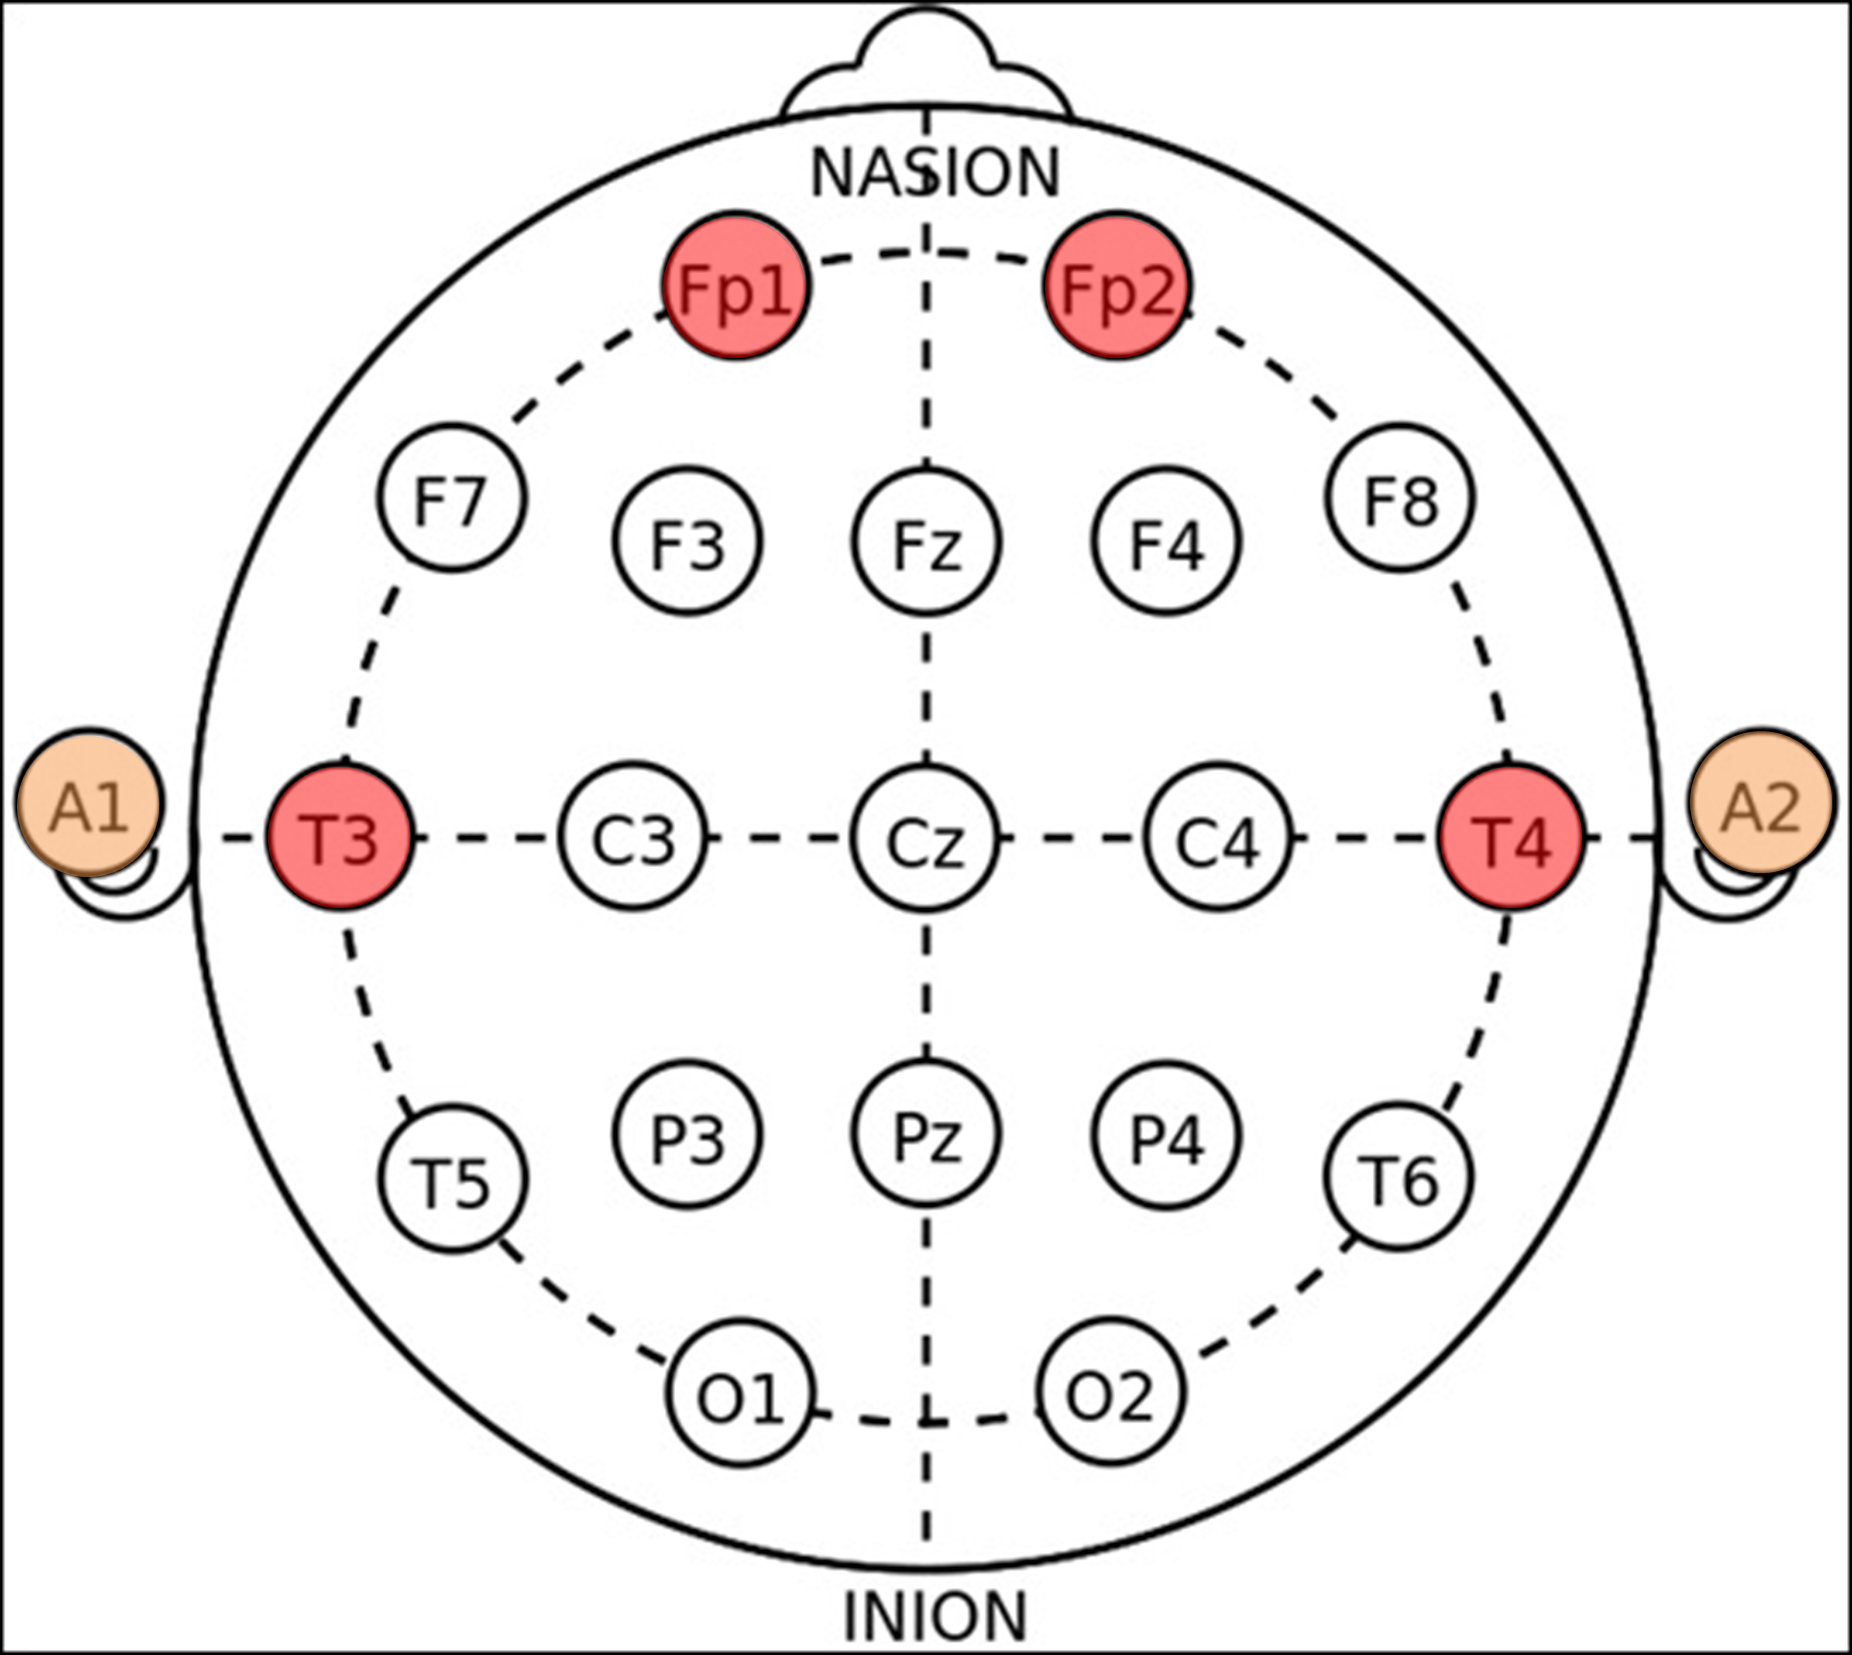
\includegraphics[width=0.35\textwidth]{pictures/elektroden-platzierungen.png}
		\caption{10-20 System mit den von uns genutzten Elektroden rot und Earclips orange gefärbt}
	\end{wrapfigure}

	Unser EEG-Gerät besteht aus einem Klettband mit Löchern für die Elektroden, einer Platine, in welche die Elektroden eingesteckt werden, und einem USB-Dongle, mit welchem die Signale der Platine kabellos empfangen werden können.

	Insgesamt haben wir zwei Earclips, die an den Ohren befestigt werden und zum Filtern von Störungen dienen, und vier Messelektroden, mit einer zeitlichen Auflösung von jeweils 200 Herz (200 Messungen pro Sekunde). Zwei dieser Elektroden haben wir auf der Stirn platziert, zwei jeweils links und rechts auf dem Schädel, etwas über dem Ohr.

	Also kriegen wir $4 * 200 = 800$ Signale pro Sekunde.
	
	Bevor wir diese in das Neuronale Netzwerk geben, verarbeiten wir sie aber erstmal mithilfe der sogenannten Fourier Transformation. Diese kann die verschiedenen zugrundeliegenden Frequenzen einer Zahlenfolge grob extrahieren, indem diese in Sinus-Kurven zerlegt wird.

	Daraus folgt ein Array (eine Liste) an Werten. Der Index bestimmt, für welche Frequenz der Wert gilt (erster Wert: 1 Herz, zweiter Wert: 2 Herz, etc.) und der Wert gibt an, womit die entsprechende Sinus-Funktion multipliziert werden muss, um die originale Funktion wiederzuerlangen. \cite{3b1b:fft}

	So lässt sich bestimmen, welche Frequenzen am stärksten vorkommen. Außerdem können dann Frequenzen herausgefiltert werden, indem die entsprechenden Indices ignoriert werden.

	Abbildung: Beispiel FFT von Sinuskurven mit 3 Hz, 5 Hz, 12 Hz

	Um die Signale in Julia empfangen, in Dateien speichern, und laden zu können, haben wir BrainFlow benutzt.

	%\begin{figure}
	%	\includegraphics{}
	%\end{figure}

	\subsubsection{Neuronales Netz}

	Ein neuronales Netzwerk besteht aus drei Teilen: dem Input Layer, den Hidden Layers und dem Output Layer. 

	Der Input ist eine Liste aus Zahlen zwischen 0 und 1. Er gibt an, welche Eingaben (Inputs) das Netzwerk bekommen soll, z. B. die Grauwerte der Pixel eines Bildes.
	
	Die Hidden Layers sind eine Ansammlung von in mehrere Layer (Schichten) unterteilten Neuronen. 
	
	Jedes Neuron besitzt eine Aktivierung (Activation), die als Zahl zwischen 0 und 1 angegeben werden kann, und einen Bias (Verzerrung), der eine beliebige Zahl sein kann. Die Neuronen verschiedener Layer sind alle durch sogenannte Gewichte (Weights) verbunden, die ebenfalls einen beliebigen Wert haben können. 

	Die Outputs sind dann lediglich die Aktivierungen der Neuronen im Output Layer.
	
	\threesub{Was ist ein neuronales Netzwerk?}

	Zuerst wollten wir die Grundstruktur eines neuronalen Netzwerkes programmieren. Ein neuronales Netzwerk besteht aus drei Teilen: dem Input Layer, den Hidden Layers und dem Output Layer.

	Der Input Layer ist nur eine Liste aus Zahlen zwischen 0 und 1. Er gibt an, welche Eingaben (Inputs) das Netzwerk bekommen soll, z. B. die Grauwerte der Pixel eines Bildes.

	Die Hidden Layers sind eine Ansammlung von in mehrere Layer (Schichten) unterteilten Neuronen. Jedes Neuron besitzt eine Aktivierung (Activation), die als Zahl zwischen 0 und 1 angegeben werden kann, und einen Bias (Verzerrung), der eine beliebige Zahl sein kann. Die Neuronen verschiedener Layer sind alle durch sogenannte Gewichte (Weights) verbunden, die ebenfalls einen beliebigen Wert haben können.  

	\threesub{Forward Pass}

	Zur Berechnung der Aktivierung eines Neurons gibt es den sogenannten Forward Pass. Dabei beginnt man im ersten Hidden Layer damit, für alle Neuronen den sogenannten Netz Input (auch net input) zu berechnen. Um den Netz Input eines Neurons zu berechnen, werden alle Aktivierungen des vorherigen Layers mit den von dem Neuron dorthin führenden Gewichten multipliziert und summiert. Der Bias ist eigentlich auch ein Gewicht, jedoch ist er mit einem Neuron verbunden, das immer die Aktivierung 1 hat.

	\begin{wrapfigure}{r}{0.4\textwidth}
		\centering
		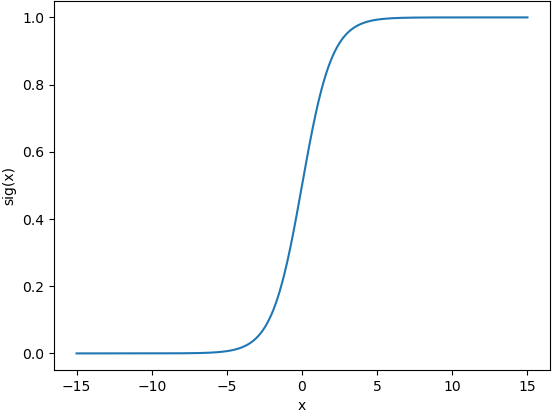
\includegraphics[width=0.4\textwidth]{pictures/sig_func.png}
		\caption{Graph der Sigmoidfunktion}
	\end{wrapfigure}

	Um aus diesem Netz Input nun die Aktivierung zu berechnen, benötigt man eine Aktivierungsfunktion, die dafür sorgt, dass die Aktivierung zwischen 0 und 1 liegt. Wir haben dafür eine Sigmoidfunktion benutzt, die eine Zahl nimmt und einen Wert zwischen 0 und 1 ausgibt. Dies wird dann für jedes Neuron in jedem Layer wiederholt. Da man aber immer die Aktivierungen des vorherigen Layers benötigt, muss man das ganze vom Input Layer zum Output Layer machen. Daher auch der Name Forward Pass. Die Interpretation der Outputs hängt von den Trainingsdaten ab. (s. Backwardpass). Die allgemeine Formel für die Aktivierung eines Neurons lautet also:
	

	{\Large
	\[
		\sig(x)=\frac{1}{1+e^{-x}}
		\]
	\[
		a_i=\sig\left({\netin}_i \right)
		\]}
	
	wobei $a_i$ = die Aktivierung des Neurons $i$ und $\netin_{i}$ = der Netzinput des Neurons $i$.

	Dies wird dann für jedes Neuron in jedem Layer wiederholt. Da man aber immer die Aktivierungen des vorherigen Layers benötigt, muss man das ganze vom Input Layer zum Output Layer machen. Daher auch der Name Forward Pass. Die Outputs sind dann lediglich die Aktivierungen der Neuronen im Output Layer. Die Interpretation dieser hängt von den Trainingsdaten ab (s. Backpropagation - Theorie). Die allgemeine Formel für die Aktivierung eines Neurons lautet also: 

	{\Large \[
		a_{j} = \sig\left(\sum_{L} (a_{L} * W_{Lj}) + b_{j}\right)
		\]}
		
	\noindent wobei $a_j$ = die Aktivierung des Neurons $j$, $L$ = der nächste Layer, $a_L$ = alle Aktivierungen des Layers $L$ , $W_{Lj}$ = alle Gewichte zwischen dem Neuron $j$ und den Neuronen des Layers $L$, und $b_j$ = der Bias des Neurons $j$.
	
	\threesub{Loss/Cost} 

	Um zu bestimmen, wie gut ein bestimmtes Neuronales Netz ist, gibt es die sogenannte Cost-Funktion (auch Loss-Funktion genannt), die mithilfe von Trainingsdaten funktioniert.
	
	Trainingsdaten bestehen aus einer Liste aus Trainingsdatensätzen. Jeder dieser Datensätze beinhaltet Inputs für das Netzwerk und die richtigen Outputs dafür. Machine Learning, das mit solchen Trainingsdaten arbeitet, wird Supervised Learning genannt.

	Die Funktion für die Cost des Output Layers und somit gesamten Netzwerkes (für einen Trainingsdatensatz) lautet wie folgt:

	{\Large \[
		C_0 = (a_L - y)^2
	\]}

	%C0 = (aL − y)2 

	\noindent wobei $C_0$ = die Cost des Output Layers, $L$ = der letzte Layer (Output Layer), $a_L$ = die Aktivierungen des Layers $L$, und $y$ = die richtigen Outputs für die Inputs, mit denen die Aktivierungen berechnet wurden. 
	
	Um die Cost zu berechnen muss man also für alle Output Neuronen die Differenz der gegebenen und der richtigen Aktivierungen bilden. Danach muss man diese Differenzen quadrieren und am Ende alle Ergebnisse aufsummieren. Dies kann man für alle Trainingsdatensätze wiederholen und von allen Costs den Durchschnitt nehmen, um die allgemeine Performance eines Netzwerkes zu überprüfen. Diese Art der Cost-Funktion wird Mean Squared Error (MSE) genannt. Zusammenfassend kann man also sagen, dass die Cost die Abweichung von den berechneten und den richtigen Outputs angibt.
	Aufgrund des Trainingsdatensatzes weiß man nun, wie der Output Layer verändert werden
	muss.

	\threesub{Backwardpass}

	Doch wie verändert man nun die Aktivierungen des Output Layers? Es müssen alle Gewichte und Biases davor angepasst werden. Um nun zu wissen, wie ein Gewicht verändert werden muss, gibt es folgende Funktion:

	\[
		\Delta W_{ij} = \epsilon * \delta_i * a_j
	\]

	wobei $\Delta W_{ij}$ = um wie viel das Gewicht $W$ zwischen den Neuronen $j$ und $i$ verändert werden muss, $\epsilon$ = die Lernrate (meist ein kleiner Wert wie 0.001), $\delta_i \approx$ die Ableitung der Cost des Neuronen $i$ im Verhältnis zum Weight $W_{ij}$, und $a_j$ = die Aktivierung des Neurons $j$. Was dabei oft verwirrend ist: $j$ bezeichnet das Neuron, welches zuerst kommt, und $i$ das Neuron, welches danach kommt (Reihenfolge im Forward-Pass), obwohl es bei $W_{ij}$ andersherum steht.

	Für den Bias wird die gleiche Formel benutzt, mit der Ausnahme, dass $a_j$ immer 1 ist und so wegfällt. Der Grund dafür liegt darin, dass der Bias, wie in der Struktur beschrieben, eigentlich nur ein Gewicht ist, das mit einem Neuron verbunden ist, welches immer eine Aktivierung von eins hat.

	Um nun $\delta_i$ für den Output Layer zu berechnen, gibt es folgende Gleichung: 

	\[
		\delta_i = \sig '\left({\netin}_i\right) * (a_i (\textrm{soll}) - a_i (\textrm{ist})) 
	\]

	wobei $\sig '(x)$ = die Ableitung von $\sig(x)$, also $\sig'(x) = \sig(x) * (1 - \sig(x))$, $\netin_i$ = der Netzinput des Neurons $i$ , $a_i(\textrm{soll})$ = die Aktivierung, die das Neuron haben sollte (also das gleiche wie $y$), und $a_i(\textrm{ist})$ = die Aktivierung, die das Neuron hat.

	Mit dieser Formel wird berechnet, welche Aktivierung das Neuron haben sollte, was an $a_i(\textrm{soll}) - a_i(\textrm{ist}))$ erkennbar ist. Die Aktivierungsfunktion mit dem Netz Input wird als Faktor mit einberechnet, da möglichst nur die Gewichte stark verändert werden sollen, die bei dem Trainingsdatensatz eine hohe Aktivierung haben, also durch diese Inputs besonders angesprochen werden. So werden zum Beispiel beim Sortieren nur die Neuronen miteinander verknüpft, die für ein bestimmtes Muster verantwortlich sind. Für die Neuronen der Hidden Layers muss man alle $\delta$'s des nächsten Layers mit den von dem Neuron dorthin führenden Weights multiplizieren und dann summieren. Dadurch werden die Änderungen, die die Aktivierungen dieser Neuronen brauchen ($\delta$), zusammengerechnet, da natürlich die Aktivierungen im nächsten Layer unterschiedliche Änderungen in dem gleichen Neuron benötigen. Durch die Multiplikation mit den dahin führenden Weights werden diese Änderungen gewichtet, da sie auf einige Neuronen größere Auswirkungen haben als auf andere. Wie beim Output Layer auch wird diese Summe noch mit $\sig'(\netin)$ multipliziert, um die Aktivierung durch bestimmte Muster angesprochener Neuronen noch weiter zu erhöhen und weniger/kaum angesprochener Neuronen zu senken, sodass die Ergebnisse besser und eindeutiger werden. Die Formel:

	{\Large \[sig'({netzinput}_i) * \sum_{L}{\left(\delta_L\ast W_{Li}\right)}\]}
		
	\noindent wobei $L$ = der nächste Layer, $\delta_L$ = alle $\delta$'s des Layers $L$, und $W_{Li}$ = alle Weights, die ein Neuron des nächsten Layers und Neuron $i$ verbinden.


	Da immer die nächsten Layer und der Output Layer benötigt werden, ergibt es Sinn, diese Optimierung beim Output Layer zu starten und dann rückwärts die \mbox{$\delta$-Werte} für jeden Layer zu berechnen und für die nächsten Berechnungen zu speichern -- daher auch der Name Backpropagation. \cite{MITNeuronale}

	\begin{figure}[h!]
		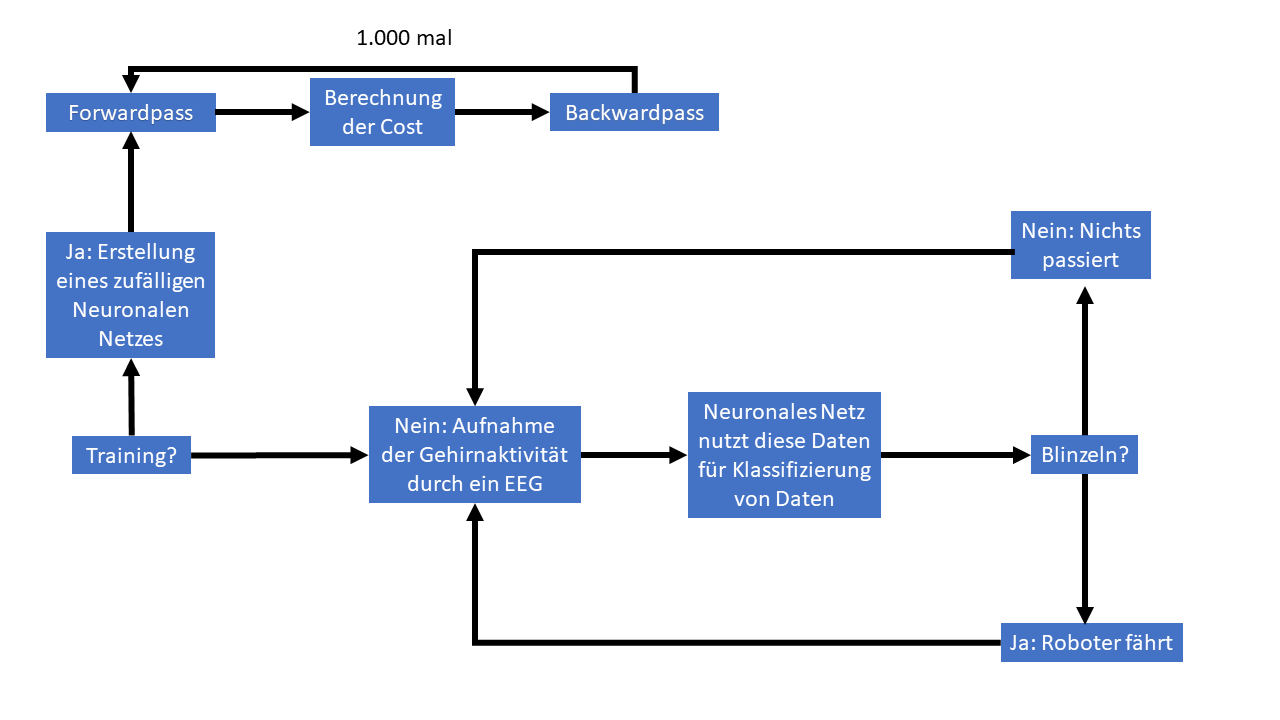
\includegraphics[width=\textwidth]{pictures/Abbildung-des-Programms.png}
		\caption{Funktionsweise des Programms}
	\end{figure}
	

	\threesub{Flux}

	Wir haben in unserem letzten Projekt bereits ein Neuronales Netzwerk mit dieser Funktionsweise selbstprogrammiert, um es besser verstehen zu können. \cite{AIComposer} Für dieses Projekt haben wir allerdings das Package Flux benutzt, welches die gleichen Ergebnisse liefern sollte, jedoch mit deutlich besserer Performance, da es sehr stark optimiert wurde.


	\subsubsection{Roboter}

	Für unseren Roboter haben wir uns entschieden, Lego Mindstorms EV3 Motoren zu benutzen, die von einem EV3-Brick gesteuert werden, der wiederum von einem Raspberry Pi 3B gesteuert wird. Der Grund dafür, dass wir keine Motoren direkt mit dem Raspberry Pi steuern, ist, dass wir schon alle Teile für einen EV3 Roboter haben. Somit müssten wir entweder neue Motoren kaufen oder passende Adapter finden, welche meist nur mit C und Python funktionieren und teuer sind.

	\begin{figure}[h!]
		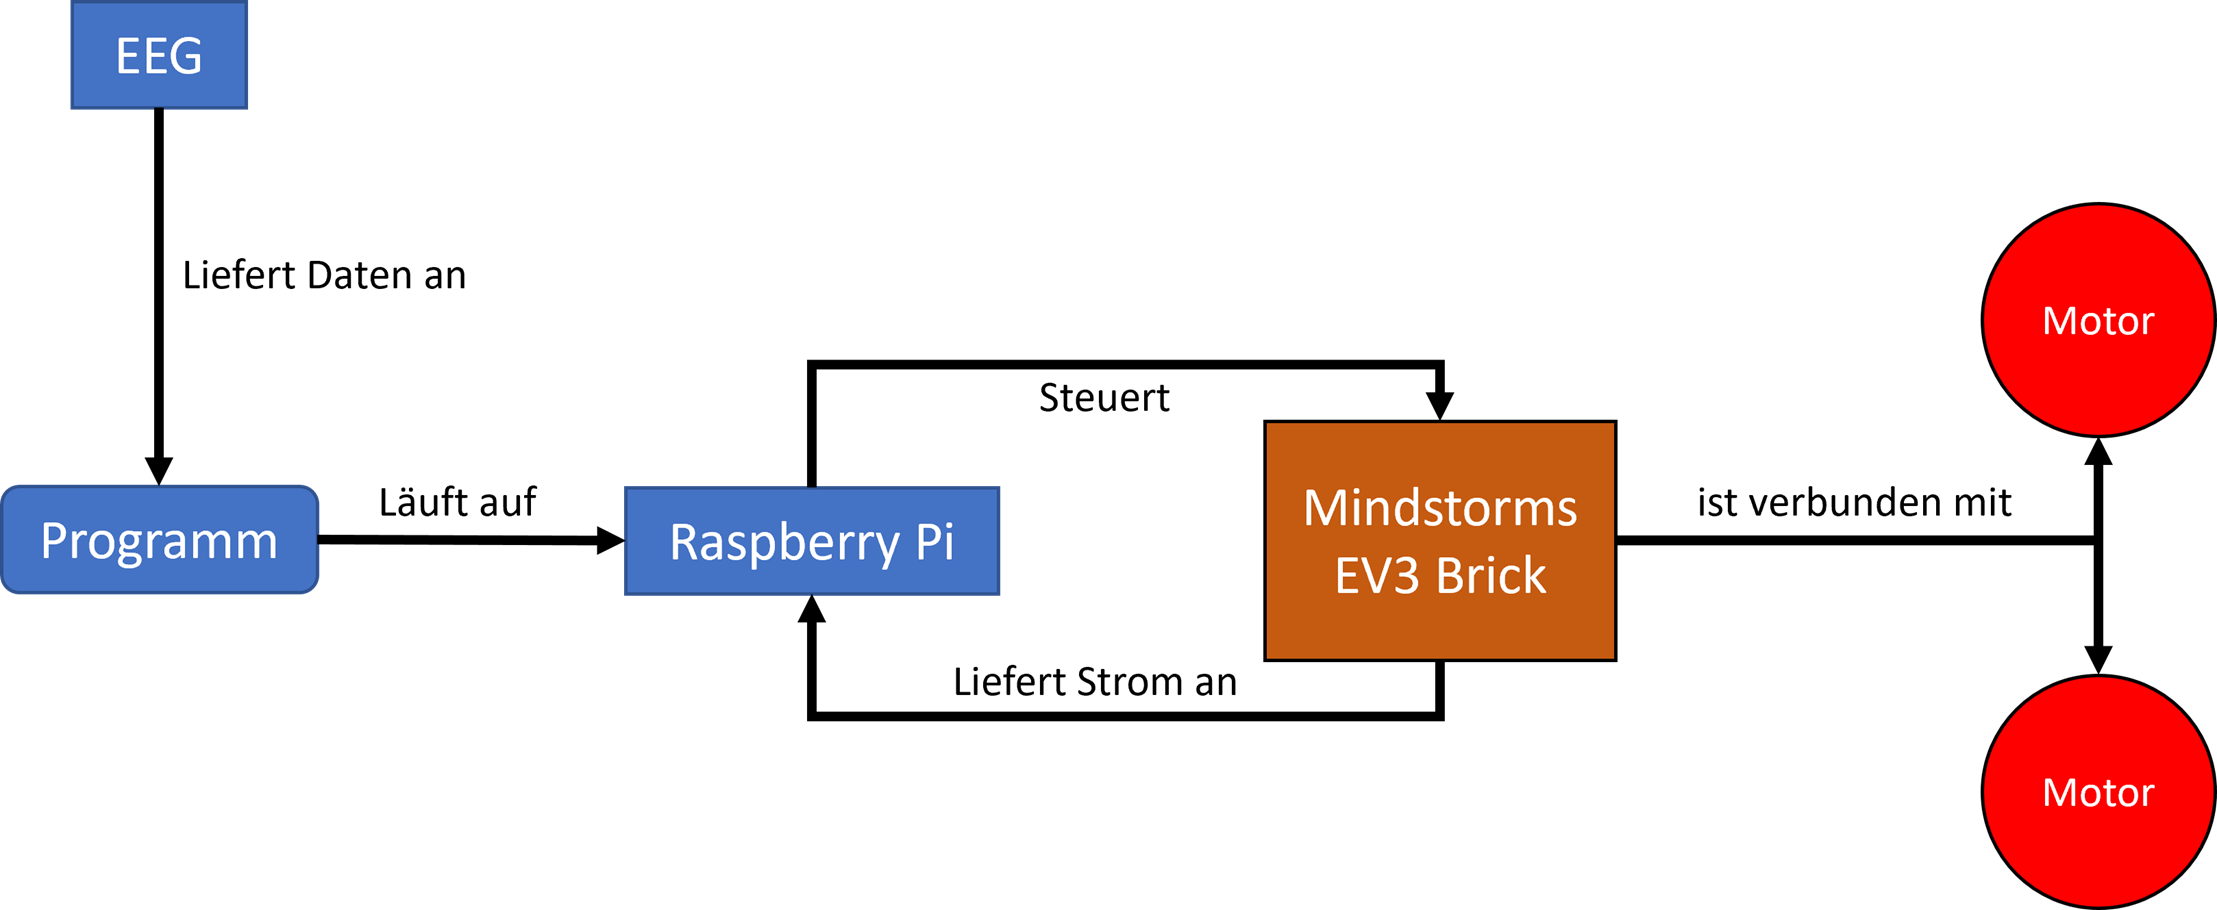
\includegraphics[width=1\textwidth]{pictures/roboter-funktionsweise.png}
		\caption{Ablauf von Gehirnaktivität zur Motorbewegung}
	\end{figure}

	Wir haben dafür das Packages ev3dev.jl benutzt, welches wir bereits für die Robotik-AG programmiert hatten. Deshalb ist der Roboter bereits fertig, obwohl das Neuronale Netz noch nicht so weit ist.

	Mehr technische Details zu der Umsetzung lassen sich beim GitHub Repository des Packages finden \cite{ev3dev}.

	\begin{figure}[h!]
		\includegraphics[width=\textwidth]{pictures/roboter-annotated.png}
		\caption{Unser Roboter (ohne Raspberry Pi, der über den EV3-Brick gehört)}
	\end{figure}

	%\newpage
	%\subsection{Funktionsweise des Programms}

	%\begin{figure}[h!]
	%	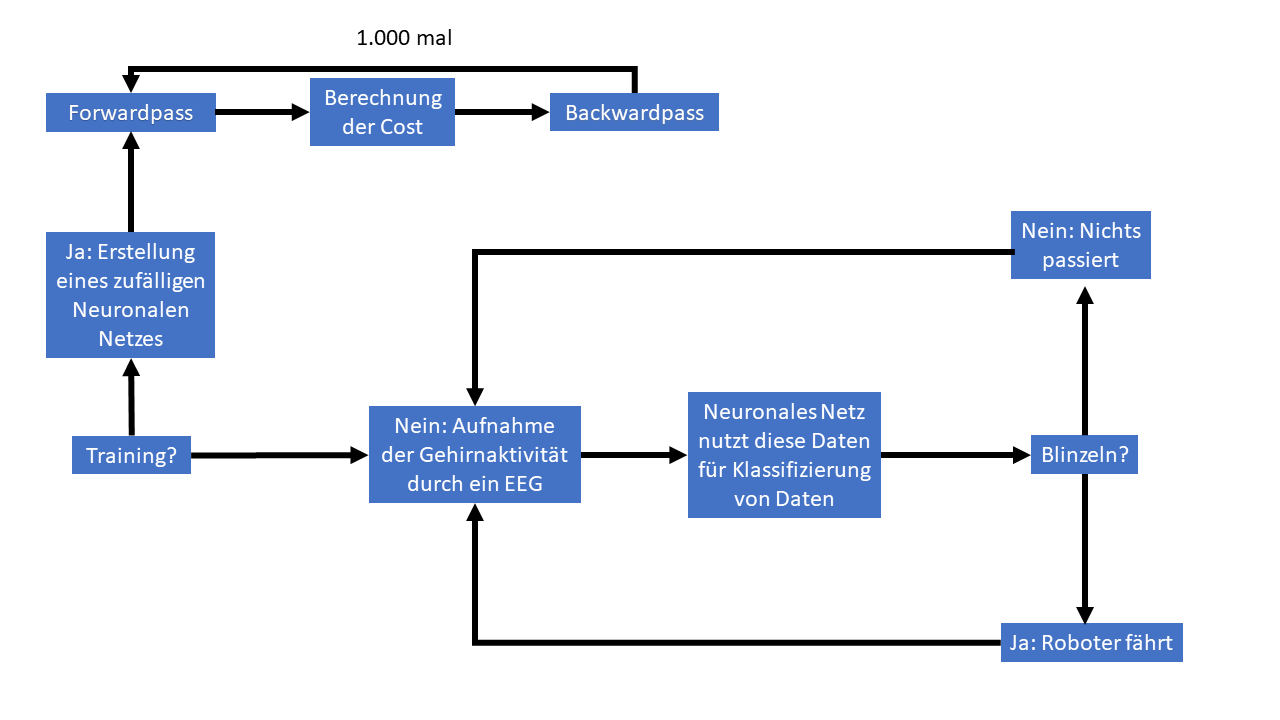
\includegraphics[width=\textwidth]{pictures/Abbildung-des-Programms.png}
	%	\caption{Funktionsweise des Programms}
	%\end{figure}
	
	\newpage

	\section{Ergebnisse}

	Zuerst haben wir versucht, eine KI zu trainieren, welche erkennen kann, ob eine Person gerade geblinzelt hat oder nicht. Diese könnte man zum Beispiel nutzen, indem man einen Roboter immer dann nach vorne fahren lässt, wenn eine Versuchsperson blinzelt.

	Wir haben uns für ein neuronales Netzwerk entschieden, welches als Input eine Sekunde an EEG-Daten nimmt, da sich die Auswirkungen von Blinzeln ungefähr für diesen Zeitraum in den EEG-Daten abbilden. 

	Als Outputs haben wir uns für zwei Neuronen entschieden. Dabei stehen die Werte jeweils für die Sicherheit des Netzwerkes, dass geblinzelt oder nicht geblinzelt wurde.

	Unsere Trainingsdaten bestehen dann aus 200 dieser Datensätzen, 100 davon mit Blinzeln und 100 ohne. Unser Netzwerk haben wir aber nur mit 90\% dieser Datensätze (180) trainiert, damit wir mit den restlichen 20 kontrollieren konnten, ob das Netzwerk auch  unbekannte Daten richtig verarbeiten kann.

	Für den Aufbau der Hidden Layer des Netzwerkes haben wir uns entschieden, da wir mehrere verschiedene Ansätze ausprobiert haben und diese Struktur konsistent die besten Ergebnisse geliefert hat.

	\begin{figure}[h]
		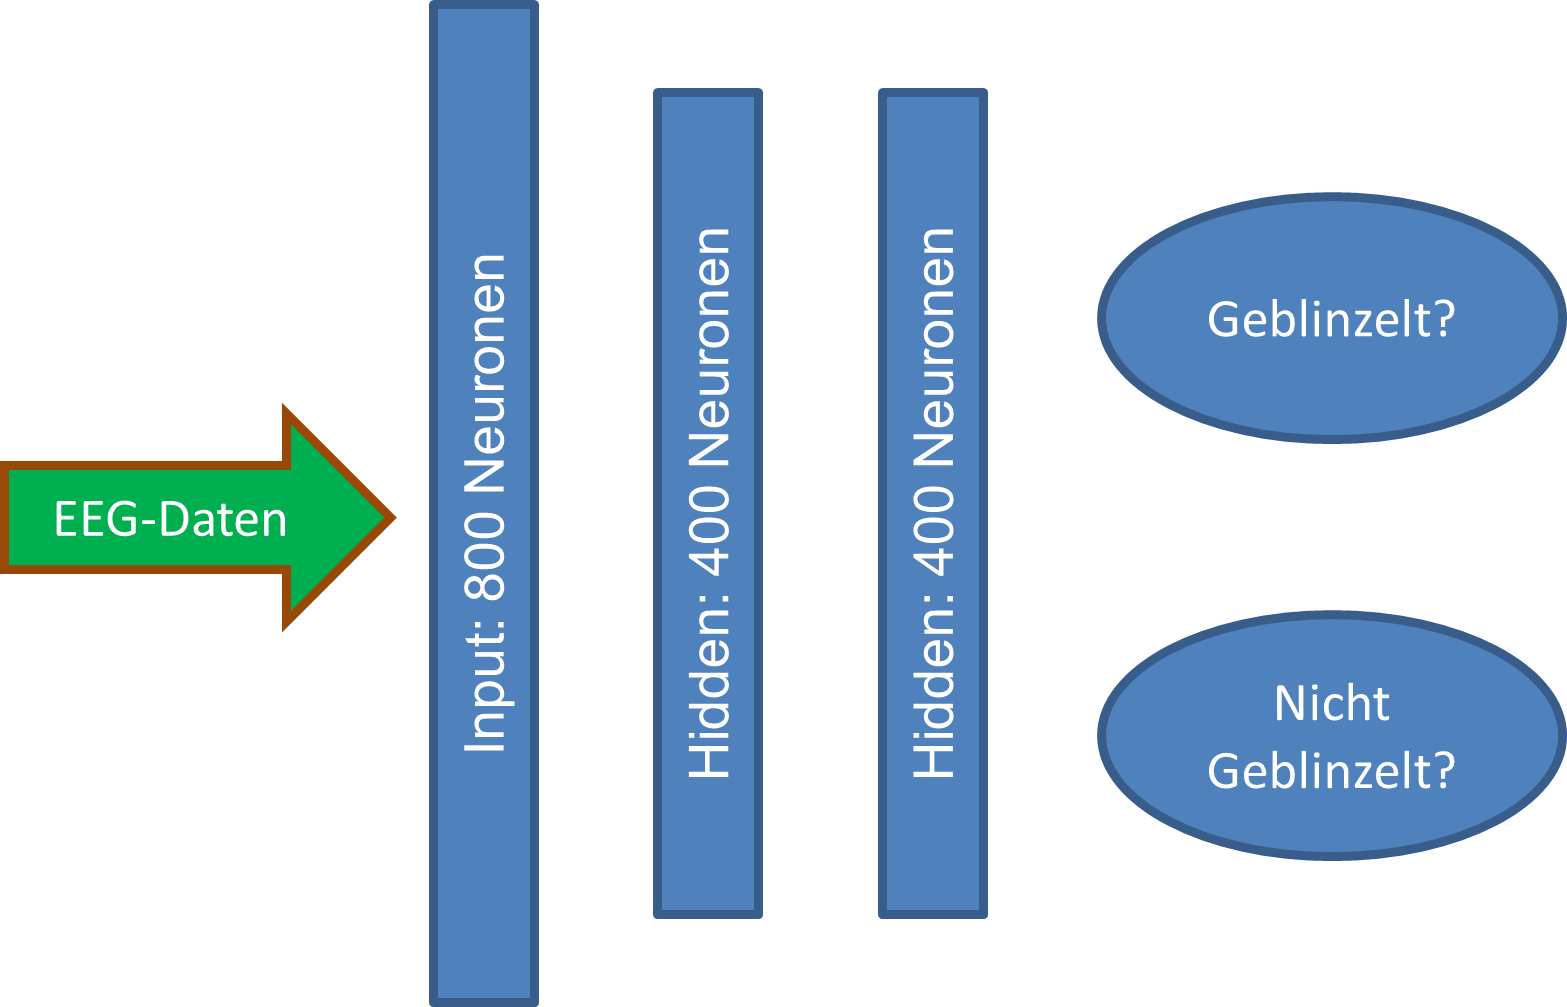
\includegraphics[width=\textwidth]{pictures/netzwerk-struktur.png}
		\caption{Struktur unseres Neuronalen Netzwerks}
	\end{figure}

	Bei dem Versuch mit Frequenzfiltern durch FFT (selbe Struktur, jedoch mit 50 Inputs, da wir auf 1 bis 50 Herz beschränkt haben) erhielten wir sehr schlechte Ergebnisse, es war kein deutlicher Unterschied zum Zufall erkennbar.

	Plot der Cost- \& Accuracy-Entwicklung!

	Ohne FFT nur mit den rohen Daten haben wir es jedoch geschafft, eine Genauigkeit von 100\% für Testdaten zu erzielen, mit denen das neuronale Netz nicht trainiert wurde.

	Plot der Cost- \& Accuracy-Entwicklung!

	Wir glauben, dass dafür die Methode unserer Datensammlung verantwortlich ist. Denn wir nehmen die EEG-Daten von Blinzeln direkt an der Stirn, über den Augen, auf. Da das Auge ein Dipol ist (zwei unterschiedlich geladenen Seiten hat) und beim Blinzeln der Augapfel sich automatisch mit der negativ geladenen Vorderseite nach oben (in Richtung der Elektroden) dreht, entsteht so ein direkter elektrischer Ausschlag – jedoch ohne eine bestimmte Frequenz.
	
	Die Frequenzen haben also keinen direkten Zusammenhang mit dem Blinzeln. Deshalb kann unser neuronales Netzwerk kein Blinzeln erkennen, wenn es nur die Stärke der Frequenzen als Inputs erhält.

	\begin{figure}[h]
		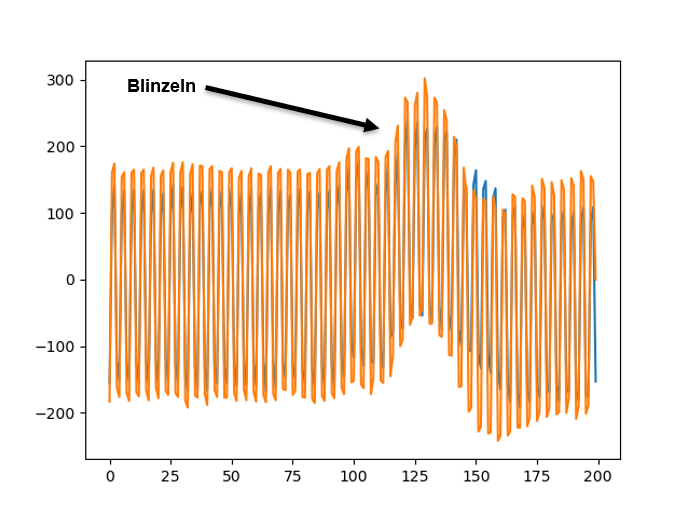
\includegraphics{pictures/blinzeln_ekp_beispiel_pyplot_annotated.png}
		\caption{Ausschnitt eines EEGs mit Blinzeln}
	\end{figure}

	\section{Diskussion}

	Das Problem mit der Anwendung von FFT wollen wir lösen, indem wir die Elektroden an einer anderen Stelle am Schädel platzieren, wahrscheinlich am Okzipitalen Kortex, da dort Alpha-Wellen (Wellen im Bereich von 7 – 13 Herz) am stärksten ausgeprägt sind und unser EEG diese am zuverlässigsten messen kann.

	Als wir das trainierte Neuronale Netzwerk für Blinzeln mit Daten testeten, die unter anderen Umständen entstanden (anderer Raum, andere Person, etc.), sank die Zuverlässigkeit der Ergebnisse drastisch, auch wenn sie besser als zufällig war.

	Grund dafür ist vermutlich, dass das Netzwerk nur mit Daten trainiert / getestet wurde, die alle kurz nacheinander von der gleichen Person unter gleichen Umständen aufgenommen wurden. 

	Um dieses Problem zu lösen, wollen wir also versuchen, mehr Trainingsdaten zu sammeln, die unter verschiedenen Bedingungen aufgenommen wurden, um unser Ziel der allgemeinen Nutzbarkeit erfüllen zu können. Außerdem könnte eine Verbesserung der Signalqualität des EEG ebenfalls zur besseren Konsistenz der Daten beitragen. Umgesetzt könnte dies werden durch z.B. die Verwendung eines Elektrodengels, bessere Platzierung der Elektroden und ein besseres Filtern von Rauschen in den Daten.

	Zudem wollen wir in Zukunft versuchen, mithilfe unseres Neuronalen Netzes bereits bei allen Menschen vorhandene, selbstkontrollierbare Gehirnaktivität zu finden und sicher zu erkennen, jedoch ohne vorherige Konditionierung. Solche Gehirnaktivität könnte z.B. der allgemeine Gedanke an \enquote{Rechts} sein, was womöglich mit erhöhter Aktivität auf der linken Hirnhälfte in Verbindung stehen könnte. 

	\section{Danksagung}

	\subsection{Finanzierung} \label{Foerderverein}

	Danke an den Förderverein \enquote{Gesellschaft der Freunde des Gymnasium Eversten e.V.} für die Finanzierung des EEG-Geräts. Alle finanzierten Teile sind in der \hyperref[Materialien]{Materialliste} mit $\star$ gekennzeichnet. 

	\subsection{Unterstützung}

	Danke an Professor Everling vom \enquote{The Brain and Mind Institute} der Western University in Kanada. \footnote{\href{https://www.uwo.ca/bmi/investigators/stefan-everling.html}{https://www.uwo.ca/bmi/investigators/stefan-everling.html}}

	Danke an Ino Saathoff, der für uns die Hülle der EEG-Platine mit seinem 3D-Drucker erstellt hat.

	Danke an Ino und Oliver Samkovskij, die zusammen mit uns den Roboter gebaut haben.

	\section{Quellen \& Referenzen}

	\printbibliography[title={Literatur/Videos}, keyword={Literatur}]

	\printbibliography[title=Programme, keyword=Programme]

\end{document}